\documentclass[12pt, a4paper]{article}
\usepackage{exercise}
\usepackage{amsmath}
\usepackage{amsfonts}
\usepackage{siunitx}
\usepackage[shortlabels]{enumitem}
\usepackage[margin=2.5cm]{geometry}
\usepackage{graphicx}
\usepackage[french]{babel}
\usepackage[justification=centering]{caption}
\usepackage[upright]{fourier}
\usepackage{tikz}
\usetikzlibrary{optics, shapes, calc}

\graphicspath{ {./rsc/} }

\sisetup{inter-unit-product=\ensuremath{{}\cdot{}}}
\renewcommand{\ExerciseHeader}
{
  \par\noindent
  \textbf{\large \ExerciseName\ \ExerciseHeaderNB\ExerciseHeaderTitle\ExerciseHeaderOrigin}%
  \par\nopagebreak\medskip
}

\renewcommand{\ExerciseName}{Exercice}

\newenvironment{conditions}
  {\par\vspace{\abovedisplayskip}\noindent\begin{tabular}{>{$}l<{$} @{${\quad}={\quad}$} l}}
  {\end{tabular}\par\vspace{\belowdisplayskip}}

\begin{document}
    \title{Exercices du Chapitre Images et Couleurs \\ \Large{Pages 327-330}}
    \author{Diego Van Overberghe}
    \date{27 Mai 2020}
    \maketitle

    \begin{Exercise}[number={11}]
        \begin{enumerate}[a.]
            \item   $\overline{OA}=-6{,}2$
            \item   $\overline{OA'}=6{,}2$
            \item   $f'=\left(\frac{1}{\overline{OA'}}-\frac{1}{\overline{OA}}\right)^{-1}=3{,}1$
            \item   $\overline{AB}=1{,}5$
            \item   $\overline{A'B'}=-1{,}5$
        \end{enumerate}
    \end{Exercise}

    \begin{Exercise}[number={14}]
        \begin{enumerate}[1.]
            \item   \begin{enumerate}[a.]
                        \item	Position de $\overline{A'B'}=5{,}2$
                        \item   L'image est réele.
                        \item   L'image est à l'envers.
                        \item   Taille de $\overline{A'B'}=1{,}6$
                        \item   $\overline{\gamma}=\frac{\overline{A'B'}}{\overline{AB}}=-1$
                    \end{enumerate}
            \item   \begin{enumerate}[a.]
                        \item	Position de $\overline{A'B'}=-1{,}9$
                        \item   L'image est virtuelle.
                        \item   L'image est à l'endroit.
                        \item   Taille de $\overline{A'B'}=2{,}8$
                        \item   $\overline{\gamma}=\frac{\overline{A'B'}}{\overline{AB}}=1{,}75$
                    \end{enumerate}
        \end{enumerate}
    \end{Exercise}

    \pagebreak

    \begin{Exercise}[number={17}]
        \begin{enumerate}[1.]
            \item	Il s'agit de la distance focale de la lentille. C'est la longeur $\overline{OF'}$, où $F'$ est le point focal.
            \item   \parbox[t][][c]{\linewidth}{\centering\begin{tikzpicture}[use optics, scale=1]
                        \draw[style=help lines, gray!75] (-7cm, -3cm) grid[step=1] (7cm,3cm);
                        %\draw[thin] (5,-1) -- (5,1) (-150,-1) -- (-150,1);
                        %\draw (7.5cm,-2.5cm) node[scale=0.5, fill=white, inner sep=1] {$F'$} (0.5cm,3cm) node[anchor=south west, scale=0.5,fill=white, inner sep=0.5] {$A'$} (-150cm,0) node[scale=0.5, anchor=north east] {A} (-150,15) node[scale=0.5, anchor=south east] {B};
                        \draw[->, very thick] (-6, -2) edge (-5, -2) -- (-6, -2) -- (-6, -1);
                        \node[lens, focal length=5cm, object height=5cm] (L) at (0,0) {};
                        \draw (-7,0) -- (7,0);
                        \draw (0,0) node[anchor=north west] {$O$} (-5.5, -2.5) node {1 cm} (-6.5, -1.5) node {1 cm} (5,-0.5) node[fill=white] {$A'$} (5,0) [black, fill=black]circle (1pt);
                    \end{tikzpicture}} \medbreak
                    \parbox{\linewidth}{\captionof{figure}{Schéma Optique de l'Appareil Photo}}
            \item   $\dfrac{1}{\overline{OA'}}=\dfrac{1}{\overline{OA}}+\dfrac{1}{f'}\iff OA'=0{,}052\ \si{m}$
        \end{enumerate}
    \end{Exercise}

    \begin{Exercise}[number={18}]
        \begin{enumerate}[1.]
            \item	Le cristallin représente la lentille.
            \item   \parbox[t][][c]{\linewidth}{\centering\begin{tikzpicture}[use optics]
                        \draw[->, thick] (-5,0) -- (5,0);
                        \node[lens, focal length=1cm] (L) at (3,0) {};
                        \draw[thick] (-4.5, 0) -- (-4.5, 0.75);
                        \draw[red] (-4.5, 0.75) -- (3, 0.75) -- (5, -0.375) (-4.5, 0.75) -- (5, -0.2);
                        \draw (4.33,0) node[anchor=south]{$F'$} (4.33,0) [black, fill=black]circle (1pt);
                    \end{tikzpicture}} \medbreak
                    \parbox{\linewidth}{\captionof{figure}{Schéma du Fonctionnement Optique de l'Œil}}
            \item   Oui, car l'image est nette au niveau de la rétine.
            \item   La distance focale doit diminuer. On voit que si $AB$ se rapproche, la droite $BB'$ devient plus pentue. Pour que le point d'interséction des rayons reste sur la rétine, le foyer image doit donc se déplacer vers le cristallin, réduisant la distance focale.
            \item   Pour mettre à point les objets très proches, l'œil peut adapter la distance focale du cristallin. Une camera ne peut pas changer la distance focale de ses lentilles mais peut changer la distance entre la lentille et la péllicule.
        \end{enumerate}
    \end{Exercise}

    \begin{Exercise}[number={19}]
        \begin{enumerate}[1.]
            \item   \begin{enumerate}[a.]
                        \item	Pour obtenir la couleur jaune à partir d'une synthèse additive, il faut des projecteurs rouge et vert.
                        \item   Il faut des projecteurs bleu et rouge.
                    \end{enumerate}	
            \item   Pour obtenir un éclairage blanc à partir des projecteurs rouge vert et bleu, il activer chaqun à 100\%.
            \item   Il est possible de reproduire toutes les couleurs à condition d'avoir des projecteurs avec une luminosité controlable.
            \item   Le modèle de synthèse mis en œuvre est la synthèse additive.
        \end{enumerate}
    \end{Exercise}

    \begin{Exercise}[number={21}]
        \begin{enumerate}[1.]
            \item	\begin{enumerate}[a.]
                        \item	La couleur de la lumière incidente est blanc.
                        \item   Les couleurs des lumières transmises sont le rouge et le vert. La couleur de la lumière absorbée est le bleu.
                        \item   La couleur de la lumière observée est le jaune.
                    \end{enumerate}
                    \begin{enumerate}[a.]
                        \item	La couleur de la lumière incidente est jaune.
                        \item   La couleur de la lumière transmise est rouge. La couleur de la lumière absorbée est vert.
                        \item   La couleur de la lumière observée est rouge.
                    \end{enumerate}
                    \begin{enumerate}[a.]
                        \item	La couleur de la lumière incidente est cyan.
                        \item   La couleur de la lumière transmise est vert. La couleur de la lumière absorbée est cyan.
                        \item   La couleur de la lumière observée est le vert.
                    \end{enumerate}
            \item   Pour répondre au a. et au c., on utilise la synthèse additive, pour répondre au b., on utilise la synthèse soustractive.
        \end{enumerate}
    \end{Exercise}

    \begin{Exercise}[number={22}]
        \begin{enumerate}[1.]
            \item	Le filtre bleu transmet le bleu, le filtre vert transmet le vert, le filtre jaune transmet le rouge et le vert, le filtre magenta transmet le rouge et le bleu.
            \item   Le filtre vert ne transmet que la lumière verte, cette lumière est aussi transmise par le filtre jaune, donc, la lumière observée à la sortie sera verte. 
            \item   L'ordre des filtres ne change pas la couleur finale, parce que le filtre transmettera toujours les mêmes couleurs, indépendament de sa position.
            \item   En superposant un filtre magenta et un filtre vert, toute les trois couleurs primaires sont diffusés, à la sortie, on ne voit que du noir.
            \item   Les couleurs vert et magneta sont dites ``complémentaires''.
            \item   La couleur complémentaire du bleu est le jaune, donc en superposant ces deux filtres, la toute la lumière sera absorbée.
        \end{enumerate}
    \end{Exercise}

    \begin{Exercise}[number={23}]
        \begin{enumerate}[1.]
            \item	Cet objet absorbe le vert.
            \item \ \\ \parbox{\linewidth}{
                        \centering\vspace{-\baselineskip}
                        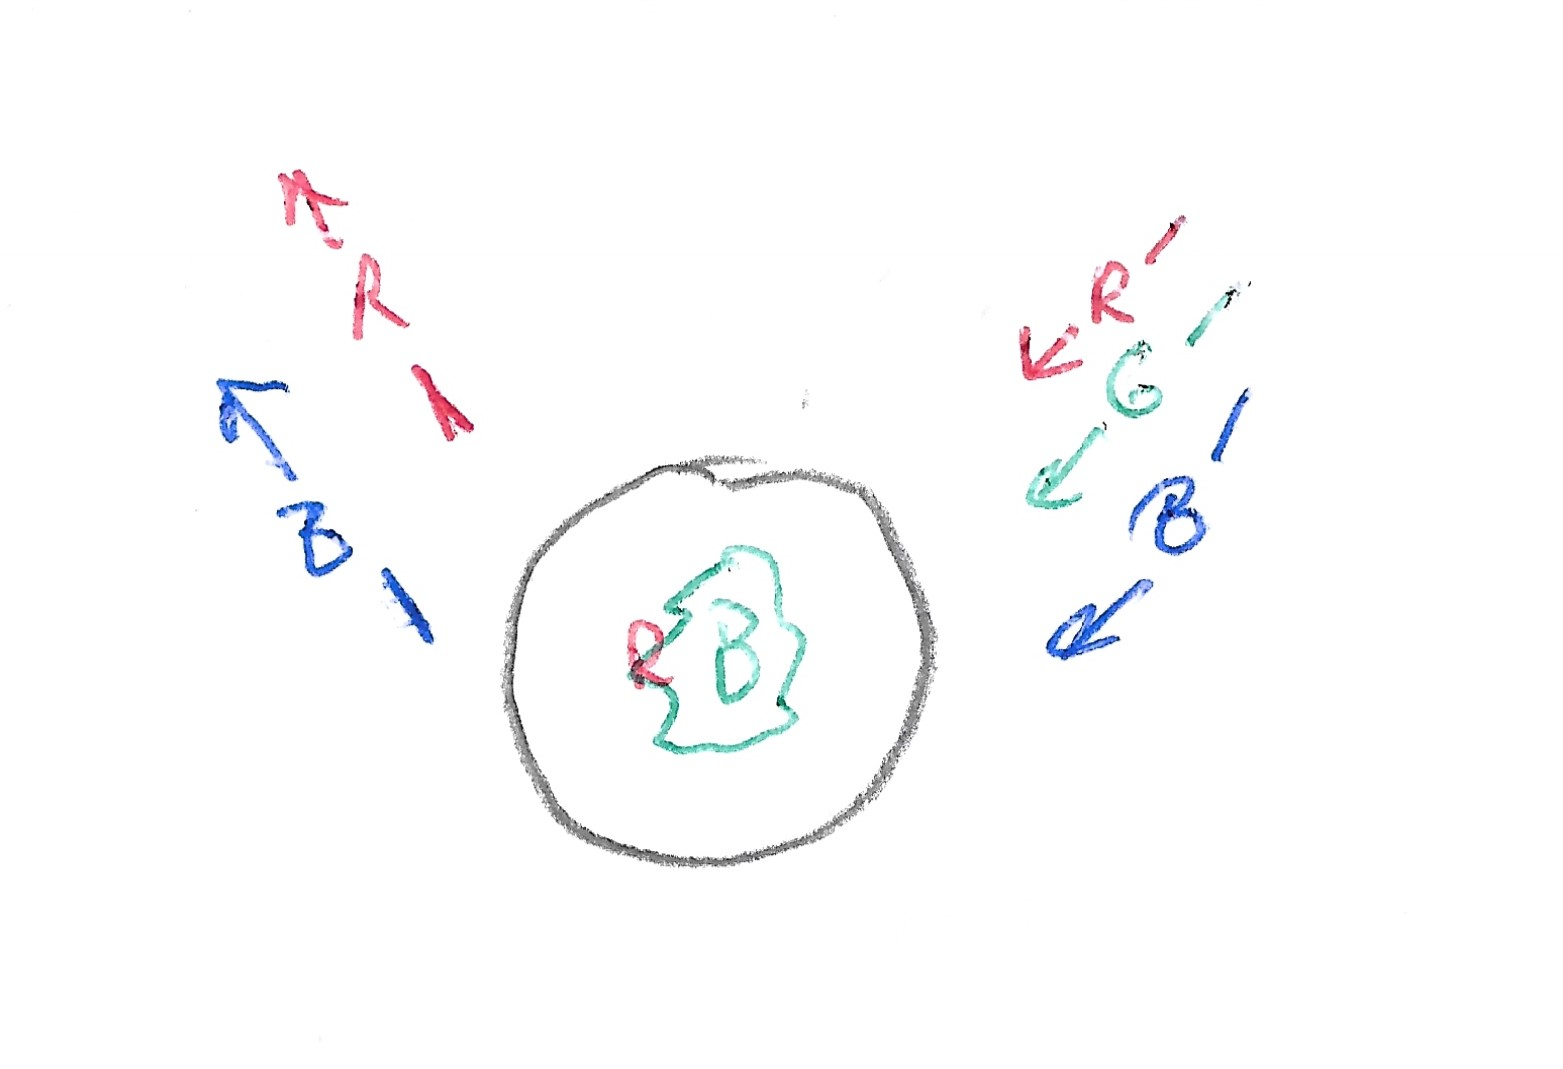
\includegraphics[width=5cm]{EX23img1.jpg}
                        \captionof{figure}{Schema Illustrant les Interactions entre l'Objet et la Lumière}
                    }
            \item   La couleur perçue est le magenta.
        \end{enumerate}
    \end{Exercise}

    \begin{Exercise}[number={24}]
        \begin{enumerate}[1.]
            \item	De gauche à droite: source de la lumière; lumière incidente; lumière transmise; lumière diffusée.
            \item   Les materieaux que rencontrent les rayons de lumière (au niveau de la torche, du filtre et de l'objet).
            \item   Le rouge, le vert et le bleu.
            \item   \begin{enumerate}[a.]
                        \item   La lumière blanche est composée de rouge, vert et bleu. Le filtre transmet la lumière verte et bleue. Le jaune est composé de rouge et vert, donc la lumière diffusée est verte.
                        \item   L'objet est donc perçu comme vert par l'observateur.
                    \end{enumerate}
        \end{enumerate}
    \end{Exercise}

    \begin{Exercise}[number={27}]
        \begin{enumerate}[1.]
            \item	{\large\textcircled{\small{a}}}$\rightarrow$ Cône bleu; {\large\textcircled{\small{b}}}$\rightarrow$ Cône vert; {\large\textcircled{\small{c}}}$\rightarrow$ Cône rouge.
            \item   Parce qu'on possède trois cônes, qui sont adaptés à détecter trois couleurs.
            \item   \begin{enumerate}[a.]
                        \item	La couleur est le bleu foncé.
                        \item   Tous les cônes sont stimulés, cependant, le cône stimulé de manière la plus intense est le cône {\large\textcircled{\small{a}}}, car il a l'intensité relative la plus élevée des trois pour cette longeur d'onde.
                        \item   Bleu foncé.
                    \end{enumerate}
            \item   Lorsque l'œil perçoit la couleur jaune, les récepteurs {\large\textcircled{\small{b}}} et {\large\textcircled{\small{c}}} sont stimulés. C'est les récepteurs résponsables de détecter les couleurs vert et rouge, les deux composants du jaune.
        \end{enumerate}
    \end{Exercise}

    \begin{Exercise}[number={29}]
        \begin{enumerate}[1.]
            \item	$\begin{aligned}[t]
                        &\quad \frac{1}{\overline{OA'}}=\frac{1}{\overline{OA}}+\frac{1}{f'} &\\
                        \iff&\quad \overline{OA'}=\left(\frac{1}{-1{,}2\times 10^{2}}+\frac{1}{30}\right)^{-1} &\\
                        \iff&\quad \overline{OA'}=40\ \si{cm}
                    \end{aligned}$
            \item   $\lvert\overline{OA}\rvert>f'\implies$ l'image est réele. \\ Comme l'image est réele, l'image est à l'envers. \\ $\overline{A'B'}=\overline{\gamma}\times\overline{AB}=\frac{\overline{OA'}}{\overline{OA}}\times\overline{AB}=\frac{40}{-1{,}2\times 10^2}\times 2{,}0 \quad \text{soit} \quad \overline{A'B'}=-0{,}67\ \si{cm}$
        \end{enumerate}
    \end{Exercise}

    \pagebreak

    \begin{Exercise}[number={33}]
        \begin{enumerate}[1.]
            \item	\parbox[t][][c]{\linewidth}{\centering\begin{tikzpicture}[use optics]
                        \draw[style=help lines, gray!75] (-5cm,-1.5cm) grid[xstep=1cm, ystep=1mm] (5cm,1.5cm);
                        \node[lens, focal length=4cm, object height=3cm] (L) at (2,0) {};
                        \draw (-5,0) -- (5,0) (-3.5, -0.9) node[scale=0.5]{1 cm} (-4.5, -0.75) node[scale=0.5]{1 mm} (2,0) node[scale=0.75, anchor=north west]{O} (-2,-0.2) node[scale=0.75]{F} (-0.5,-0.2) node[scale=0.75]{A} (-0.5,0) -- (-0.5,1.2mm) [->] (-4,-0.8) edge (-3, -0.8) [->] (-4,-0.8) -- (-4, -0.7) ;
                        
                    \end{tikzpicture}} \medbreak
                    \parbox{\linewidth}{\captionof{figure}{Représentation du Système Optique}}
            \item   $\overline{OF}=4\ \si{cm}\quad\overline{OA}=2{,}5\ \si{cm}\quad\overline{AB}=1{,}2\ \si{mm}$
            \item   $\dfrac{1}{\overline{OA'}}=\dfrac{1}{\overline{OA}}+\dfrac{1}{\overline{OF}}\iff\overline{OA'}=1{,}5\ \si{cm}$
            \item   $\gamma=\dfrac{\overline{OA}}{\overline{OA'}}=\dfrac{\overline{AB}}{\overline{A'B'}}=2{,}67$ \medbreak $\overline{A'B'}=\gamma\overline{AB}=3{,}2\ \si{mm}$
        \end{enumerate}
    \end{Exercise}

    \begin{Exercise}[number={35}]
        \begin{enumerate}[1.]
            \item	Sans éclairage bleu, on pourrait confondre le drapeau de l'Italie et du Mali.
            \item   Aucun éclairage, ou pas de vert et pas de bleu, c'est-à-dire un éclairage uniquement rouge.
            \item   Un filtre jaune.
        \end{enumerate}
    \end{Exercise}

    \begin{Exercise}[number={36}]
        \begin{enumerate}[1.]
            \item	\parbox[t][][c]{\linewidth}{\centering\begin{tikzpicture}[use optics]
                        \draw (-5,0) -- (5,0);
                        \node[lens, focal length=5cm] (L) at (0.8,0) {};
                        \draw (0.8,0) node[anchor=south west, scale=0.75]{O} (-4,0) node[anchor=north, scale=0.75]{A} -- (-4, 0.75) node[anchor=south, scale=0.75]{B} [dashed] (4,1) -- (4,-1) (4,0) node[anchor=south west, scale=0.75]{$A'$} (4, -0.5) node[anchor=west, scale=0.75]{$B'$};
                        \draw[red] (-4, 0.75) -- (0.8,0.75) -- (4,-0.5) (-4, 0.75) -- (4,-0.5) (-4,0.75) -- (0.8, -0.5) -- (4, -0.5);
                    \end{tikzpicture}}
                    \parbox{\linewidth}{\captionof{figure}{Représentation du Système Optique}}
            \item   $\dfrac{1}{\overline{OA'}}=\dfrac{1}{\overline{OA}}+\dfrac{1}{\overline{OF}}\iff OA'=51\ \si{mm}$
            \item   $\gamma=-0{,}028$
            \item   $\overline{A'B'}=-51\ \si{mm}$
            \item   Il faut déplacer l'objectif pour que le point focal $F'$ soit positionné sur le capteur. \\ $\overline{OF'}=50\ \si{mm}$
        \end{enumerate}
    \end{Exercise}

    \pagebreak

    \begin{Exercise}[number={39}]
        \begin{enumerate}[1.]
            \item	\parbox[t][][c]{\linewidth}{\centering\begin{tikzpicture}[use optics]
                        \draw (-5cm,0) -- (20mm,0);
                        \node[lens, focal length=15.7mm] (L) at (0,0) {};
                        \draw (14mm,0) node[anchor=south west, scale=0.75]{$F'$} [black, fill=black] circle (1pt);
                        \coordinate (P) at (-5,0.75);
                        \coordinate (Q) at (-5,-0.75);
                        \coordinate (R) at (-5,0.33);
                        \coordinate (S) at (-5,-0.33);
                        \draw[red] (P) -- ($(L.north)!(P)!(L.south)$) -- (L.east focus) (Q) -- ($(L.north)!(Q)!(L.south)$) -- (L.east focus) (R) -- ($(L.north)!(R)!(L.south)$) -- (L.east focus) (S) -- ($(L.north)!(S)!(L.south)$) -- (L.east focus);
                    \end{tikzpicture}} \medbreak
                    \parbox{\linewidth}{\captionof{figure}{Représentation du Système Optique}}
            \item   $f'=15{,}2+0{,}50=15{,}7\ \si{mm}$
            \item   $f'_\text{min}=14{,}7\ \si{mm}$ \quad $\dfrac{1}{\overline{OA'}}=\dfrac{1}{\overline{OA}}+\dfrac{1}{OF'}\iff\overline{OA}_\text{minimum net}=44{,}7\ \si{cm}$
        \end{enumerate}
    \end{Exercise}

    \begin{Exercise}[number={41}]
        \begin{enumerate}[1.]
            \item	Le filtre {\Large\textcircled{\small{A}}} est bleu, il diffuse et transmet le bleu et absorbe les autres couleurs. \smallbreak Le filtre {\Large\textcircled{\small{B}}} est jaune, c'est-à-dire il diffuse et transmet le jaune (rouge et vert), et absorbe le bleu. \smallbreak Le filtre {\Large\textcircled{\small{C}}} est rouge, il diffuse et transmet le rouge, et absorbe les autres couleurs, le bleu et le vert. \smallbreak 
                        Le filtre {\Large\textcircled{\small{D}}} est vert, il diffuse et transmet le vert, et absorbe les autres couleurs, le jaune (rouge et vert).
            \item   L'adjectif ``soustractif'' est utilisé parce que ce type de synthèse fonctionne en enlevant (soustrayant) au blanc toutes sortes de couleurs.
            \item   Le profil spéctral de la lumière transmise par un filtre magenta serait comme celui de la lumière blanche, avec un ``trou'' au milieu, puisque le vert est absorbé.
        \end{enumerate}
    \end{Exercise}
\end{document}